\section{Auswertung}
\label{sec:Auswertung}

%AUFGABENTEIL 1
\subsection{Verifizierung der Funktionsweise des Lock-In-Verstärkers}
Die Spannungsverläufe werden für die Phasenverschiebungen \varphi = 0\,°, 90\,°, 180\,°, 270\,°, 315\,°
gespeichert und in Abbildung 6a bis e dargestellt.
%Screenshots
\begin{figure}[H]
\centering
\begin{subfigure}{0.48\textwidth}
  \centering
  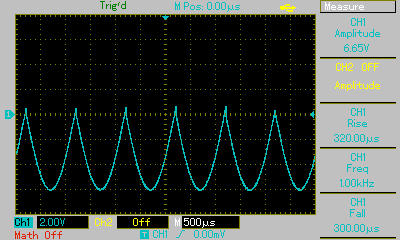
\includegraphics[height=4.3cm]{MAP010.png}
  \caption{Spannungsverlauf bei \varphi = 0°}
\end{subfigure}
\begin{subfigure}{0.48\textwidth}
  \centering
  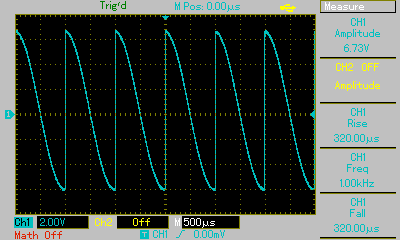
\includegraphics[height=4.3cm]{MAP011.png}
  \caption{Spannungsverlauf bei \varphi = 90°}
\end{subfigure}
\begin{subfigure}{0.48\textwidth}
  \centering
  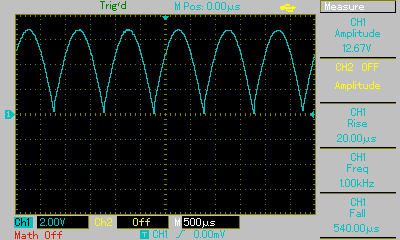
\includegraphics[height=4.3cm]{MAP013.png}
  \caption{Spannungsverlauf bei \varphi = 180°}
\end{subfigure}
\begin{subfigure}{0.48\textwidth}
  \centering
  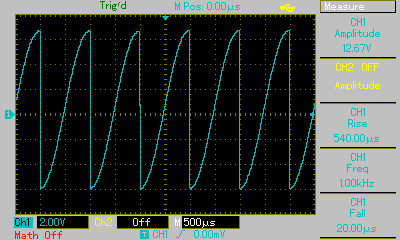
\includegraphics[height=4.3cm]{MAP014.png}
  \caption{Spannungsverlauf bei \varphi = 270°}
\end{subfigure}
\begin{subfigure}{0.48\textwidth}
  \centering
  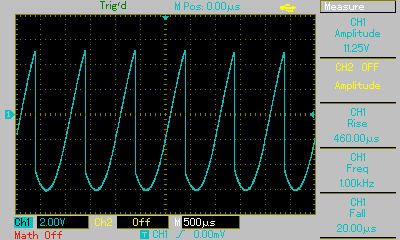
\includegraphics[height=4.3cm]{MAP015.png}
  \caption{Spannungsverlauf bei \varphi = 315°}
\end{subfigure}
\caption{Die Drillachse und Positionen der Holzpuppe}
\label{fig:versuche}
\end{figure}

Die Phasenverschiebung $\varphi$ und die Amplitude der Ausgangsspannung $U_\text{out}$ 
sind in Tabelle 1 zu sehen. In Abbildung 7 sind diese gegeneinander aufgetragen.


%Tabelle1
\begin{table}[H]
\centering
\caption{Messdaten der Ausgangspannung $U_\text{out}$ in Abhängigkeit der Phase}
\label{tab:data2}
\begin{tabular}{c c c c c c}
\toprule
$\varphi$ \:/\: ° & $\varphi$\:/\:rad  & $U_\text{out} \:/\: \si{\volt}$ & $\varphi$ \:/\: ° & $\varphi$\:/\:rad   & $U_\text{out} \:/\: \si{\volt}$\\
\midrule
0  & 0,000 & -4,0 & 105 & 1,833 & 0,5 \\
15 & 0,262 & -4,0 & 120 & 2,094 & 1,5 \\
30 & 0,524 & -3,8 & 135 & 2,356 & 2,9 \\
45 & 0,785 & -3,1 & 150 & 2,618 & 3,8 \\
60 & 1,047 & -2,0 & 165 & 2,880 & 4,3 \\
75 & 1,309 & -0,8 & 180 & 3,142 & 4,3 \\
90 & 1,571 & 0,0 & & & \\
\bottomrule
\end{tabular}
\end{table}

%Plot 1
\begin{figure}[H]
  \centering
  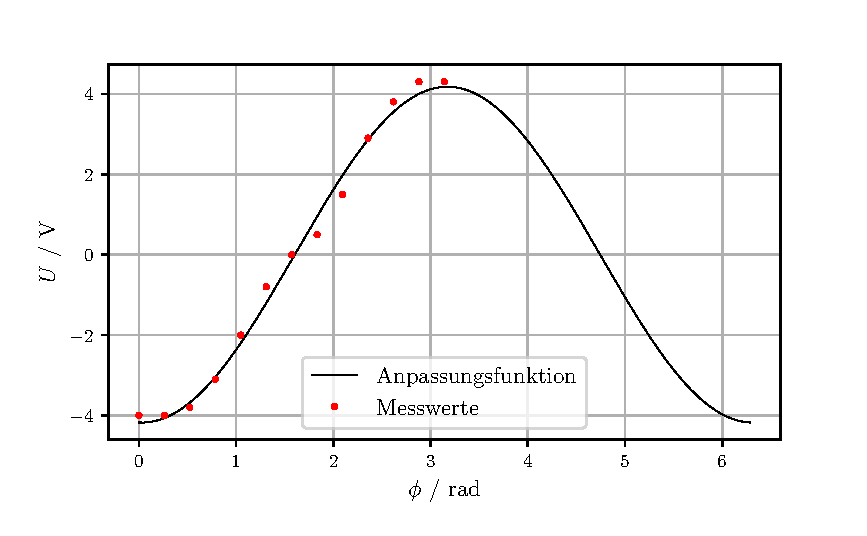
\includegraphics{plot1.pdf}
  \caption{Ausgangsspannung $U_\text{out}$ in Abhängigkeit der Phasenverschiebung $\varphi$.}
\end{figure}

Die Anpassungsfunktion ist nach Gleichung (2) eine cos-Funktion der Form
\begin{align*}
U = a\:\text{cos} (bx + c) + d.
\end{align*}
Die Parameter $a,b,c,d$ ergeben sich mit Python 3.7 zu
\begin{align*}
a &= (4,34 \pm 0,24)\,\si{\volt}, \\
b &= (0,93 \pm 0,09), \\
c &= (3,16 \pm 0,14), \\
d &= (0,22 \pm 0,19)\,\si{\volt}.
\end{align*}
Nach Gleichung (2) ergibt sich aus dem Parameter $a = \frac{2 U_\text{0}}{\pi}$ für
\begin{align*} 
U_\text{0} = (6,8 \pm 0,4)\,\si{\volt}.
\end{align*}

Die Phasenverschiebung $\varphi$ und die Amplitude der Ausgangsspannung $U_\text{out}$ 
mit zugeschaltetem Störsignal
sind in Tabelle 2 zu sehen. In Abbildung 8 sind diese gegeneinander aufgetragen.

%Tabelle2
\begin{table}[H]
\centering
\caption{Messdaten der Ausgangspannung $U_\text{out}$ in Abhängigkeit der Phasenverschiebung $\varphi$}
\label{tab:data3}
\begin{tabular}{c c c c c c}
\toprule
$\varphi$ \:/\: ° & $\varphi$\:/\:rad  & $U_\text{out} \:/\: \si{\volt}$ & $\varphi$ \:/\: ° & $\varphi$\:/\:rad   & $U_\text{out} \:/\: \si{\volt}$\\
\midrule
0  & 0,000 & -4,4 & 105 & 1,833 & 0,2 \\
15 & 0,262 & -4,3 & 120 & 2,094 & 1,3 \\
30 & 0,524 & -4,1 & 135 & 2,356 & 2,5 \\
45 & 0,785 & -3,5 & 150 & 2,618 & 3,5 \\
60 & 1,047 & -2,3 & 165 & 2,880 & 3,9 \\
75 & 1,309 & -1,0 & 180 & 3,142 & 4,0 \\
90 & 1,571 & -0,4 & & & \\
\bottomrule
\end{tabular}
\end{table}

%Plot 2
\begin{figure}[H]
  \centering
  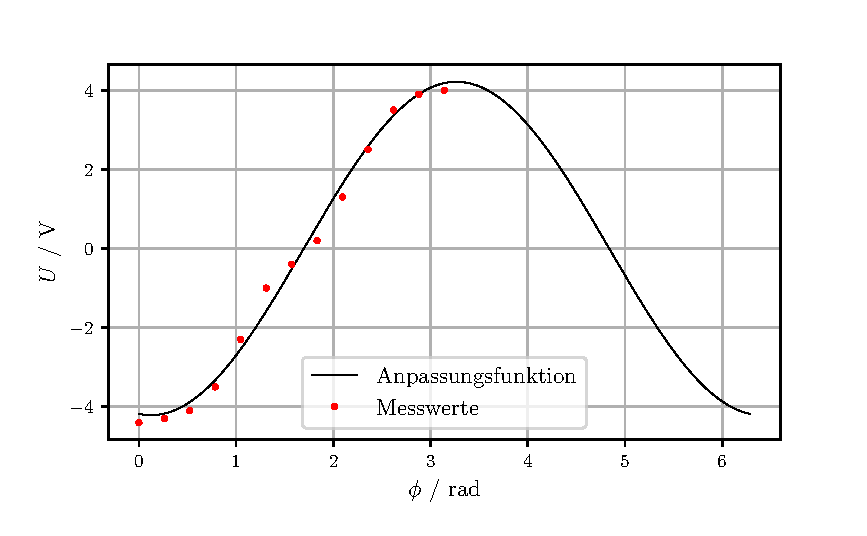
\includegraphics{plot2.pdf}
  \caption{Ausgangsspannung $U_\text{out}$ in Abhängigkeit der Phasenverschiebung $\varphi$
  bei zugeschaltetem Störsignal.}
\end{figure}

Die Anpassungsfunktion ist analog zur ersten Messreihe nach Gleichung (2) eine cos-Funktion der Form
\begin{align*}
U = a\:\text{cos} (bx + c) + d.
\end{align*}
Die Parameter $a,b,c,d$ ergeben sich mit Python 3.7 zu
\begin{align*}
a &= (4,36 \pm 0,24)\,\si{\volt}, \\
b &= (0,92 \pm 0,09), \\
c &= (3,19 \pm 0,14), \\
d &= (-0,14 \pm 0,19)\,\si{\volt}.
\end{align*}
Nach Gleichung (2) ergibt sich aus dem Parameter $a = \frac{2 U_\text{0}}{\pi}$ für
\begin{align*} 
U_\text{0} = (6,8 \pm 0,4)\,\si{\volt}.
\end{align*}

%AUFGABENTEIL 2
\subsection{Überprüfung der Rauschunterdrückung mithilfe eines Photodetektors}
Die Lichtintensität $U$ des Photodetektors und der Abstand $r$ zwischen Diode und Detektor
sind in Tabelle 3 und in Abbildung 9 zu sehen.

%Tabelle 3
\begin{table}[H]
\centering
\caption{Messdaten der Lichtintensität $U$ in Abhängigkeit des Abstands $r$}
\label{tab:data4}
\begin{tabular}{c c c c}
\toprule
$r$\:/\:\si{\centi\meter}& $U$\:/\:\si{\volt} & $r$\:/\:\si{\centi\meter}& $U$\:/\:\si{\volt} \\
\midrule
6  & 12.67 & 45 & 0.21 \\
10 &  6.34 & 50 & 0.19 \\
15 &  3.96 & 55 & 0.16 \\
20 &  3.17 & 60 & 0.12 \\
25 &  0.64 & 65 & 0.10 \\
30 &  0.43 & 70 & 0.09 \\
35 &  0.35 & 75 & 0.01 \\
40 &  0.27 & 80 & 0.01 \\
\bottomrule
\end{tabular}
\end{table}

%Plot 3
\begin{figure}[H]
  \centering
  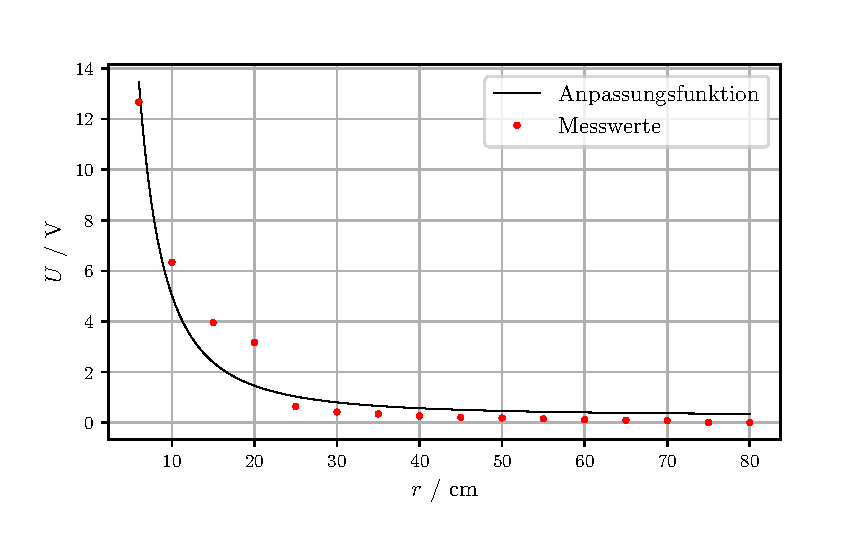
\includegraphics{plot3.pdf}
  \caption{Lichtintensität $U$ des Photodetektors in Abhängigkeit des Abstands $r$.}
\end{figure}

Die Funktion wird mit
\begin{align*}
U = a \frac{1}{x^{2}} + b
\end{align*}
angenähert.
Die Parameter der Anpassungsfunktion ergeben sich mit Python 3.7 zu
\begin{align*}
a &= (474,96 \pm 29,42)\si{\volt\centi\meter\squared},\\
b &= (0,27 \pm 0,22)\si{\volt}.
\end{align*}
Da sich die Lichtintensität in den letzten beiden Messungen nicht verändern und
diese generell zu sehr fluktuiert, wird
angenommen, dass für den maximalen Abstand $r_\text{max} = 80\,\si{\centi\meter}$
nicht mehr hauptsächlich die LED für die Lichtintensität verantwortlich ist, sodass
für $r_\text{max}$ die Intensität $U_\text{min} = 0,01\,\si{\volt}$ festgehalten wird.